\section{Database}
Vi har i vores system valgt at bruge to forskellige databaser, hvoraf de også er forskellige typer.
\\
Vi har været vant til fra studiet at bruge databaser af typen SQL, som f.\@eks.\ MS-SQL. Dog har vi i dette projekt
gået i en anden retning, og har valgt at bruge en MySQL database, samt en ElasticSearch database.
\subsection{Valg af database}
Vores valg stod imellem MySQL/MariaDB, MongoDB og ElasticSearch. Grunden til dette er at de anvender strukturer og
kompabilitet med den type teknologier vi anvender. Vi ville ikke kunne anvende en MS-SQL database, da dette er kompatibelt
med microsoft teknologier som eksempelvis sproget C\#.
\\\\
I vores situation, hvor vi har anvendt PHP til vores backend, giver MySQL/MariaDB rigtig god mening da det er kompatibelt med PHP,
og MariaDB er desuden også gratis. ElasticSearch er gratis at implementere da det er open-source, dog kræver det en server.
\\\\
Vores valg faldt på at anvende både MySQL og ElasticSearch.
\\
Grunden til at vi valgte af bruge MySQL, var at vi har noget nødvendig data som skal gemmes. Når man uploader et API giver det god mening
for os, at disse data bliver gemt på en MySQL database, så vi dermed kan pulle data fra det gemte API når vi har behov for det.\\
Vi har desuden også en ekstern MySQL database til rådighed som vi allerede betalte for inden projektperioden, ellers ville vi nok have anvendt en gratis version
af MySQL eller MariaDB.
\\\\
Grunden til vi valgte at bruge ElasticSearch til at gemme data fra API endpoints og ikke de andre typer databaser, var at da vi laver et statistik program
som skal hente data på tværs af forskellige tabeller, ville vi undgå at lave en masse kald til databasen og joine data sammen.
\\
Meget af grunden bunder derfor i performance boost til systemet, hver gang der skal hentes og indexeres data.
\\
ElasticSearch er primært lavet til indexere, søge og hente data meget effektivt og vinder derfor klart på performance ift.\ MySQL\@. 
\\\\
Der hvor ElasticSearch taber sammenlignet med de andre databaser, er at det oprindeligt er lavet som en search engine og ikke en decideret database.
\\Dvs.\ man får ikke den samme sikkerhed, som de andre tilbyder.
\subsection{ElasticSearch}
ElasticSearch er en næsten real-time search engine som er bygget på Apache Lucene, som er et søge API.\
ElasticSearch er bygget op omkring et Cluster, som er en liste af nodes, hvor en node er en server der gemmer data. Clustered indexere så dataen og gør det søgbart\footnote{https://www.elastic.co/guide/en/elasticsearch/reference/current/setup-repositories.html}.
ElasticSearch gør også brug af index, som er en liste af dokumenter, der har samme karakteristika og er skrevet i JSON format.
\\
Ved større index kan de dele et index op i shards og et shard er et fuldt funktionelt index. Det gør man kan skalere data horisontalt.
\\\\
Vi har Figur~\ref{fig:elasticsearch-arkitektur} forsøgt at skitsere den generelle opbygning af en typisk ElasticSearch server, og relationer mellem cluster, nodes og dokumenter.
\\\\
\begin{figure}[here]
    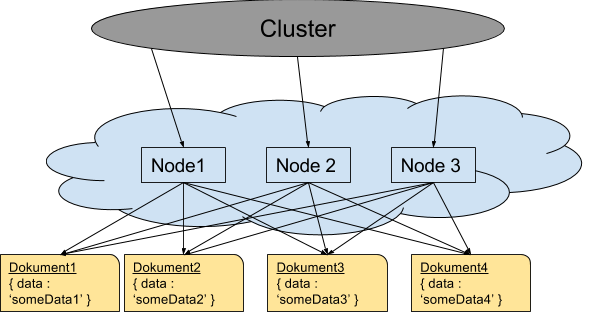
\includegraphics[scale=0.7]{ElasticSearch_arkitektur}
    \caption{Skitsering af ElasticSearch}
    \label{fig:elasticsearch-arkitektur}
\end{figure}
\subsection{Normalisering}
Når vi gemmer informationer omkring API'er, gemmer vi dem i en tabel der hedder \textit{Apis}. Denne tabel indeholder kolonnerne: Id, Index, Type og URL, se Tabel~\ref{table:api-tabel}, for visualisering af strukturen på tabellen.
\\\\
OBS! Data og struktur i tabellen er kun for eksemplets skyld, og er ikke en reel kopi af den originale tabel.
\begin{table}[here]
    \centering
    \begin{tabular}{|l|l|l|l|l}
        \cline{1-4}
        id & index  &  type &  url &  \\ \cline{1-4}
        1 & Ordbogen & antal\_søgninger\_2011 & http://ordbogen.com/api/searches\_year\_2011 &  \\ \cline{1-4}
        2 & Ordbogen & antal\_søgninger\_2012 & http://ordbogen.com/api/searches\_year\_2012 &  \\ \cline{1-4}
        3 & Ordbogen & antal\_søgninger\_2013 & http://ordbogen.com/api/searches\_year\_2013 &  \\ \cline{1-4}
    \end{tabular}
    \caption{Apis tabel}
    \label{table:api-tabel}
\end{table}

I vores overvejelser omkring normalisering har vi tænkt over hvorvidt denne tabel skal følge alle normalformer (0-3).
\\
Der opstår dog problemer ved 3. normalform som siger at \textit{"3NF kræver, at et felt \textbf{kun} er afhængig af primærnøglen.
Selvom alle felterne i en tabel overholder 2NF eller at primærnøglen slet ikke er sammensat, så kan der være tilfælde, hvor indholdet af et felt kan bestemmes alene udfra et andet felt i tabellen, som ikke selv er en del af primærnøglen."}\footnote{http://www.eksperten.dk/guide/234}
\\\\
Hvis vi kigger på Tabel~\ref{table:api-tabel} kan url'en udledes ud fra typen, da disse to felter er unikke. Det samme gælder for typen der kan udledes fra url'en.
\\
En løsning på dette ville være at lave endnu en tabel med type og url, samt en fremmednøgle med relation fra \textit{Apis} tabellen til denne nye tabel, så et id og index peger på en fremmednøgle i tabellen med type og url.
\\\\
Grunden til vi ikke valgte denne løsning var at vi synes det var for meget arbejde i forhold til hvad det ville give os.
\\
Vi vurderede i dette tilfælde at data strukturen var så simpel at det ikke gav mening at ofre tid for pænere struktur i form af at opfylde 3. normalform, men at vente med at opdele tabellen til hvis der kom flere kolonner.
